The Large Hadron Collider (LHC) is a particle accelerator consisting of a 27 km ring, designed to collide protons at high energy. Located outside of Geneva, Switzerland and buried about 100 m undergound, it consists of a ring of superconducting magnets which are used to accelerate opposing beams of protons - or lead ions - which collide at the center of one of the various detectors located around the LHC ring which record the result of these collisions. These detectors include two general purpose detectors, ATLAS and CMS, which are designed to make precision measurements of a broad range of physics phenomenon, and two more specialized experiments, LHCb and ALICE, which are optimized to study b-quarks and heavy-ion physics, respectively.

The LHC first began running in 2009 at a proton-proton center of mass energy of $\sqrt{s} = 2$ TeV. This was increased to 7 TeV in 2010-2011, and again increased to 8 TeV in 2012. The period from 2009 to 2012 is known as Run 1, and data collected during this period was used in discovering the Higgs Boson. The LHC began running again in 2015, and collected data at an increased energy of $\sqrt{s} = 13$ TeV until 2018, a period referred to as Run 2. 

Protons are fed into the LHC via a chain of accelerators, which accelerate the protons to higher and higher energies until they are injected into the main ring. This process is summarized in figure \ref{fig:AccChain}. Protons extracted from a tank of hydrogen are fed into a linear accelerator, LINAC2, where they reach an energy of 50 MeV. From there, they enter a series of three separate circular accelerators, before being injected into the main accelerator ring at an energy of 450 GeV. Within the main ring protons are seperated into two seperate beams moving in opposite directions, and their energy is increased to their full collision energy. Radiofrequency cavities are used to accelerate these particles and sort them into bunches. From 2015-2018, these bunches consisted of around 100 billion protons each with an energy of 6.5 TeV per proton, which collided at a rate of 40 MHz, or every 25 ns. 

\begin{figure}[H]
\centering
   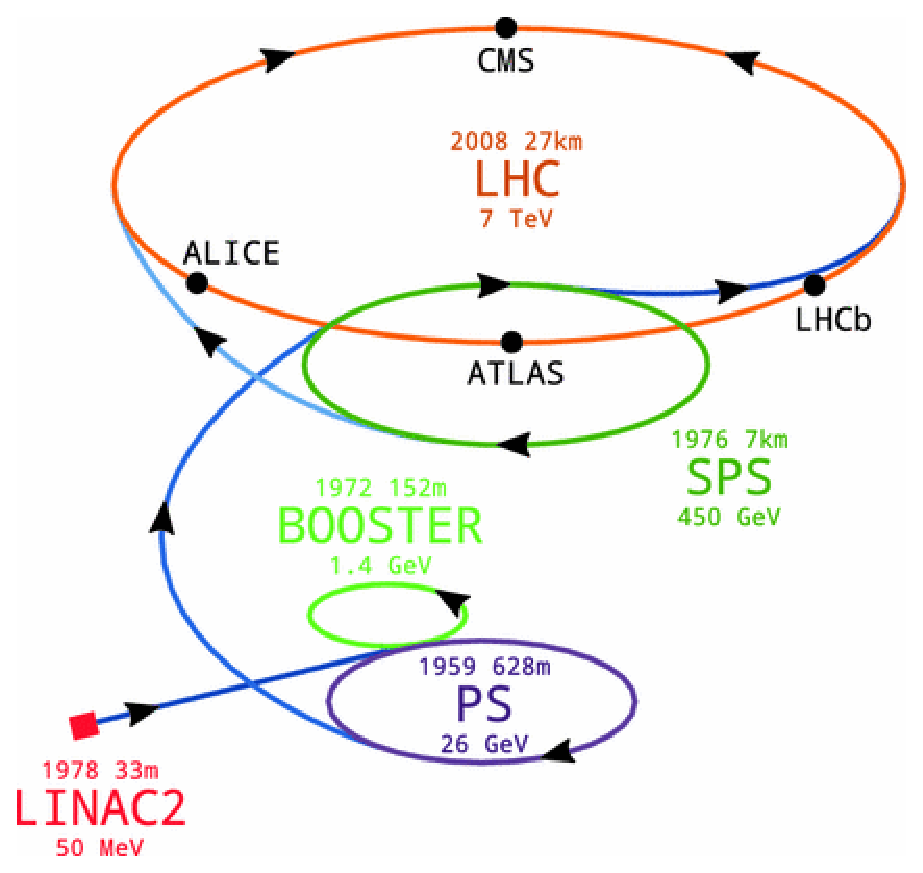
\includegraphics[width=0.7\linewidth]{figures/lhc/AccChain.eps}
\caption{A summary of the accelerator chain used to feed protons into the LHC \cite{accChainFig}.}
\label{fig:AccChain}
\end{figure}

Because these proton bunches consist of a large number of particles, each bunch crossing consists of not just one, but several direct proton-proton collisions. The additional interactions that occur in each bunch crossing, $\mu$, is known as pileup. During Run 2, the average pileup was around $\left\langle\mu\right\rangle$ = 35, with values typically ranging between 10 and 70.

The amount of data collected by the LHC is measured in terms of luminosity, which is the ratio of the number of events detected per unit time, $\frac{dN}{dt}$, and the interaction cross-section, $\sigma$. 

\begin{equation}                                                                                                                                
        \label{eq:lumiDef}                                                                                                                      
        \mathcal{L} = \frac{1}{\sigma}\frac{dN}{dt}
\end{equation}

The design luminosity of the LHC is $10^{34}\ cm^{-2}s^{-1}$, however the LHC has acheived a luminosity of over $2\times 10^{34}\ cm^{-2}s^{-1}$. The total luminosity is then this instantaneous luminosity integrated over time.

\begin{equation}
        \label{eq:intLumi}      
        \mathcal{L}_{int} = \int\mathcal{L}dt
\end{equation}

The integrated luminosity collected by the ATLAS detector as of the end of 2018 is around 140 $fb^{-1}$, exceeding the expected integrated luminosity of 100 $fb^{-1}$. This luminosity is obtained using the LUCID-2 detector \cite{LUCID2} for the primary luminosity measurements using the van der Meer (vdM) method. \cite{Balagura_2021}. This involves varying the location of one of the proton beams and observing how the collision rate is effected.
                                            
                                         
